\documentclass[a4paper,12pt]{article}
\usepackage[utf8]{inputenc}
\usepackage[french]{babel}
\usepackage[T1]{fontenc}
\usepackage[top=2cm,bottom=2cm,left=2cm,right=2cm]{geometry}
\usepackage{graphicx}
\usepackage{wrapfig}
\usepackage{url}

\begin{document}

\begin{titlepage}
	\begin{center}
		\Large{Année universitaire 2016-2017}\\
		\Large{Université de Caen Normandie}\\[1cm]
		
		\huge{Rapport sur la création de la grammaire arithmétique}\\
		\vspace{3cm}
		
		Théo Sarrazin
		
	\normalsize{\textit{ ~ L2 Informatique}}\\
		\medskip
		\vspace{2cm}
				
	\end{center}
\end{titlepage}

\tableofcontents
\newpage

\section{Lex}
	
	Comme nous avons pu le voir, les regles de lex sont définis par des tokens, chaques tokens étant associés à un expression régulière. 

	\subsection{Les tokens}

		Dans le cadre d'un grammaire arithmétique nous avons besoin de différents tokens : 
		\begin{itemize}
			\item Number : le token qui va reconnaitre les nombres
			\item Plus : le token qui va reconnaitre le signe +
			\item Minus : le token qui va reconnaitre le signe -
			\item Times : le token qui va reconnaitre le signe *
			\item Divide : le token qui va reconnaitre le signe /
			\item LParen : le token qui va reconnaitre la parenthèse gauche
			\item RParen : le token qui va reconnaitre la parenthèse droite
		\end{itemize}

		Pour être reconnnu par Lex ces tokens sont stockés dans un tuple \textbf{tokens} 

	\subsection{Les expressions régulières}

		A chacun des tokens précédents, nous devons associer une expression régulière pour que Lex puisse reconnaitre les tokens.
		Pour cela, nous devons simplement créer une variable de la forme t\_NomDuToken, est qui prend comme valeur l'expression régulière à associer à ce token.

		Pour le token Number, nous utilisons l'expression suivante : \textbf{\"\\b+\"}, le \textbf{\"\\b\"} signifiant n'importe quel chiffre compris entre 0 et 9 de plus le \textbf{+} signifie répété une ou plusieur fois. En effet un nombre est une suite de chiffre.

		Pour les six autres tokens, nous utilisons simplement le signe qui doit correspondre au token (+ pour le token Plus, - pour le token Minus, etc...)
	
		\begin{figure}[h!]
			\begin{center}
				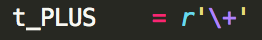
\includegraphics[scale=1]{imgs/exp_regex}
				\caption{Exemple de création d'une expression régulière}
			\end{center}
		\end{figure}


	\subsection{Fonctions et variables supplémentaires}

		De plus, pour l'utilisation de Lex, nous pouvons définir une variable \textbf{t\_ignore} qui va preciser les éléments à ne pas prendre en compte, dans notre cas la variable vaut \textbf{" \t"}, nous ignorons donc les espaces et les tabulations.

		Nous pouvons aussi définir une fonction \textbf{t\_newline(t)}, qui prend un token en paramètre et qui va être utilisée pour matcher tous les retours à la lignes grâce à l'expression régulière \textbf{\"\\n+\"}, de plus cette fonction va ajouter pour chaque ligne trouvé 1 à l'attribut \textbf{lineno}, qui contient le nombre de lignes.

		Pour finir un autre fonction peut être utilisée, la fonction \textbf{t\_error(t)}, qui prend elle aussi on token en paramètre et qui va être appelée par le lexer à chaque token non reconnue par notre lexer. Cette fonction va afficher un message d'erreur puis ignorer le token grâce à l'instruction \textbf{t.lexer.skip(1)}, t étant le token courrant grâce au quel on recupère le lexer. 

\section{Yacc}

	\subsection{Création de la grammaire}

		Pour fonctionner Yacc à besoin de différentes règles de grammaires, chaques règles definissants comment peuvent s'"assembler" les différents tokens reconnus pour Lex.

		Pour definir des règles nous devons créer des fonctions nommer de la façons suivante : \textbf{p\_NomDeLaRegle}. Cette fonction doit contenir une docstring definissant les regles à respecter.

		\begin{figure}[h!]
			\begin{center}
				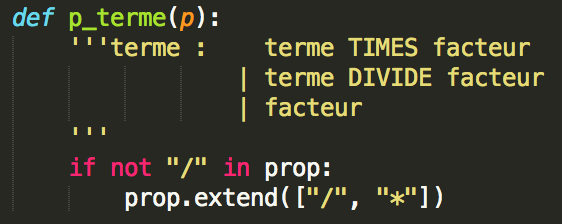
\includegraphics[scale=1]{imgs/exp_grammaire_yacc}
				\caption{Exemple d'une règle de grammaire de Yacc}
			\end{center}
		\end{figure}

		Voici nos différentes règles : 
		\begin{itemize}
			\item expression : correspond à une somme/soustraction de deux expressions. Une expression pouvant aussi être terme.
			\item terme : correspond à une multiplication/division de deux termes. Un terme pouvant aussi être un facteur.
			\item facteur : correspond à un nombre, une expression entre parenthèse ou - un facteur.
		\end{itemize}

		De plus, chacune de ces fonctions ajoute des propositions à une variable \textbf{prop} afin de les afficher par la suite dans notre IDE.

	\subsection{Création du parser}

		Par la suite, nous devons appliquer nos règles sur du contenu, pour cela nous avons créés une fonction \textbf{parse}, qui prend en paramètre le code à parser. Par la suite, cette fonction créée le lexer (en faisant appelle à Lex), puis créée le parser (en faisant appelle à Yacc), pour finir elle revoit les listes des propostions afin de pouvoir les ajouter à les listes des propostions de notre IDE.

\end{document}